\section{平行高斯信道}
\label{sec:gcc-parallel}

设发送端同时掌握三条互不干扰的线路，噪声方差分别是$1$、$2$、$5$，但三条线路共用一个功率预算$5$。功率应当平均分给三条线路，全部给最安静的那条，还是另有更好的分法？分法确定以后，三条线路合起来每次能送多少比特？

\paragraph{模型}
设$k$为固定的正整数，$\sigma_1^2,\dots,\sigma_k^2>0$。每次使用信道，发送端送出一个向量$\bm{x}_i=(x_{i,1},\dots,x_{i,k})\in\mathbb{R}^k$，接收端得到
\begin{equation}
 Y_{i,j}=x_{i,j}+Z_{i,j},\qquad j=1,\dots,k,\quad i=1,\dots,n ,
 \label{eq:gcc-parallel}
\end{equation}
其中全部噪声$Z_{i,j}$相互独立，$Z_{i,j}\sim\mathcal{N}(0,\sigma_j^2)$，并且与消息独立。第$j$个分量的噪声方差$\sigma_j^2$不随时刻改变。这样的信道称为\term{平行高斯信道}（parallel Gaussian channel）。

满足功率约束$P$的$(M,n)$码要求每条码字在所有时刻与所有分量上的总能量不超过$nP$：
\begin{equation}
 \sum_{i=1}^{n}\sum_{j=1}^{k}x_{i,j}(m)^2\leq nP,\qquad m=1,\dots,M .
 \label{eq:gcc-parallel-power}
\end{equation}
码率仍是$\frac1n\log_2M$，单位是比特每次向量使用。图~\ref{fig:gcc-parallel-model}画出$k=3$的情形。

\begin{BookInlineFigure}
 \centering
 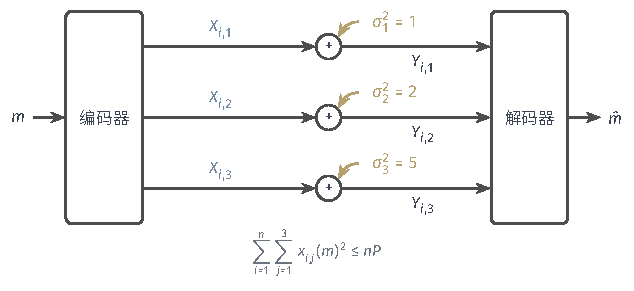
\includegraphics[width=107mm]{figures/07-probability/06-channel-coding/tikz/gcc-parallel-model/figure.pdf}
 \caption{$k=3$的平行高斯信道。第$i$次使用时，向量输入的三个分量（蓝）分别加上方差为$1,2,5$的独立噪声（黄）；三个分量和全部$n$次使用共享同一个能量预算$nP$。}
 \label{fig:gcc-parallel-model}
\end{BookInlineFigure}

\paragraph{单次使用的上界}
与标量情形一样，先在单次使用上优化。设随机输入向量$\bm{X}$的分量为$X_1,\dots,X_k$，平均能量$\mathbb{E}\lVert\bm{X}\rVert_2^2\leq P$，它与噪声向量$\bm{Z}$独立，输出$\bm{Y}=\bm{X}+\bm{Z}$。记第$j$个分量的功率为$P_j=\mathbb{E}[X_j^2]$，它们的和不超过$P$。

引理~\ref{lem:gcc-output}的证明对向量逐字成立：$\bm{Y}$有密度，$h(\bm{Y})$有限，并且
\[
 I(\bm{X};\bm{Y})=h(\bm{Y})-h(\bm{Z}) .
\]
噪声分量独立，所以$h(\bm{Z})$等于各$h(Z_j)$之和。由第~\ref{chap:information-measures}章熵的链式法则和条件化不增加熵，联合微分熵不超过各分量微分熵之和：
\[
 h(\bm{Y})\leq\sum_{j=1}^{k}h(Y_j) .
\]
每个分量的方差不超过$P_j+\sigma_j^2$，对每个分量用引理~\ref{lem:gcc-max-entropy}，得到
\begin{equation}
 I(\bm{X};\bm{Y})\leq\sum_{j=1}^{k}\bigl(h(Y_j)-h(Z_j)\bigr)\leq\sum_{j=1}^{k}\frac12\log_2\Bigl(1+\frac{P_j}{\sigma_j^2}\Bigr) .
 \label{eq:gcc-parallel-upper}
\end{equation}

这个上界可以取到：让各分量独立，$X_j\sim\mathcal{N}(0,P_j)$。此时各$Y_j$独立，次可加性取等号；每个$Y_j$是方差$P_j+\sigma_j^2$的高斯变量，熵上界也取等号。于是单次使用的问题化为一个只关于功率分配$(P_1,\dots,P_k)$的有限维问题。

\subsection{注水分配}
\label{sec:gcc-waterfilling}

要求解的是
\begin{equation}
 \max_{P_1,\dots,P_k}\ \sum_{j=1}^{k}\frac12\log_2\Bigl(1+\frac{P_j}{\sigma_j^2}\Bigr)
 \quad\text{s.t.}\quad P_j\geq0,\quad\sum_{j=1}^{k}P_j\leq P .
 \label{eq:gcc-allocation}
\end{equation}

\paragraph{边际收益}
先看每个分量多分一点功率能多得多少。第$j$项对$P_j$的导数是
\[
 \frac{\partial}{\partial P_j}\,\frac12\log_2\Bigl(1+\frac{P_j}{\sigma_j^2}\Bigr)=\frac{1}{2\ln2}\cdot\frac{1}{\sigma_j^2+P_j} .
\]
它随$P_j$增大而减小，并且在$P_j=0$处等于$1/(2\ln2\,\sigma_j^2)$：噪声越小的分量，第一份功率越值钱。于是分配应当从最安静的分量开始；它的边际收益随投入下降，降到与次安静分量的起始值相等时，再同时投入两者，使两者的边际收益保持相等，依此类推。最优时，所有分到功率的分量边际收益相同，没分到功率的分量起始收益不高于这个公共值。

\paragraph{乘子条件}
把上面的直观写成严格的最优性条件。目标函数是凹函数，约束是线性的，并且$P>0$时$P_j=P/(2k)$严格满足所有不等式约束。由卷五的凸优化理论，KKT条件对最优解既必要又充分，可参考\BookChapterRef{chap:constrained-optimality}{卷五第17章“约束问题的最优性”}。引入预算约束的乘子$\mu\geq0$与非负约束的乘子$\eta_j\geq0$，KKT条件是
\[
 \frac{1}{2\ln2}\cdot\frac{1}{\sigma_j^2+P_j}=\mu-\eta_j,\qquad \eta_jP_j=0,\qquad \mu\Bigl(P-\sum_{j}P_j\Bigr)=0 .
\]

目标函数关于每个$P_j$严格递增，预算不会留有剩余，所以$\sum_jP_j=P$且$\mu>0$。记$\nu=1/(2\ln2\,\mu)$。若$P_j>0$，则$\eta_j=0$，由第一式得$\sigma_j^2+P_j=\nu$；若$P_j=0$，则$\eta_j\geq0$，由第一式得$1/\sigma_j^2\leq1/\nu$，即$\sigma_j^2\geq\nu$。两种情形合并为$P_j=\max\{\nu-\sigma_j^2,0\}$。

\begin{theorem}[注水分配]
\label{thm:gcc-waterfilling}
设$P>0$，$\sigma_j^2>0$。问题~\eqref{eq:gcc-allocation}的唯一最优解是
\begin{equation}
 P_j=(\nu-\sigma_j^2)^{+},\qquad j=1,\dots,k,
 \label{eq:gcc-waterfilling}
\end{equation}
其中$(t)^{+}=\max\{t,0\}$，水位$\nu$是方程$\sum_{j=1}^{k}(\nu-\sigma_j^2)^{+}=P$的唯一解。平行高斯信道的信息容量是
\begin{equation}
 C(P)=\sum_{j=1}^{k}\frac12\log_2\Bigl(1+\frac{(\nu-\sigma_j^2)^{+}}{\sigma_j^2}\Bigr)
 =\sum_{j:\,\sigma_j^2<\nu}\frac12\log_2\frac{\nu}{\sigma_j^2} .
 \label{eq:gcc-parallel-capacity}
\end{equation}
\end{theorem}

\begin{proof}
函数$\nu\mapsto\sum_j(\nu-\sigma_j^2)^{+}$连续、不减，在$\nu\leq\min_j\sigma_j^2$时为零，在$\nu>\min_j\sigma_j^2$时严格递增且趋于无穷，所以方程有唯一解$\nu>\min_j\sigma_j^2$。由此定义的$P_j$非负、总和为$P$；取$\mu=1/(2\ln2\,\nu)$，$P_j>0$时取$\eta_j=0$，$P_j=0$时取$\eta_j=\mu-1/(2\ln2\,\sigma_j^2)\geq0$，KKT条件全部满足，所以它是最优解。目标函数是各分量严格凹函数之和，因而在可行集上严格凹，最优解唯一。代入目标函数，活跃分量上$1+P_j/\sigma_j^2=\nu/\sigma_j^2$，即得式~\eqref{eq:gcc-parallel-capacity}。
\end{proof}

式~\eqref{eq:gcc-waterfilling}称为\term{注水}（water-filling）分配。把第$j$个分量画成底部高度为$\sigma_j^2$的一格容器，往这排容器里倒总量为$P$的水，水面在各格中齐平，高度就是$\nu$；每格的水深就是分给它的功率。底部高于水面的格子一滴水也没有。类比的对应是：底部高度对应噪声方差，水的总量对应预算，水面齐平对应边际收益相等。类比只描述分配规则，水深与容量的关系仍要回到对数公式。

\paragraph{例：三条线路}
回到本节开头的问题：$\sigma^2=(1,2,5)$，$P=5$。把噪声方差从小到大排列，先假设只有最安静的$a$个分量活跃，由$\sum_{j\leq a}(\nu-\sigma_j^2)=P$解出
\[
 \nu_a=\frac{1}{a}\Bigl(P+\sum_{j=1}^{a}\sigma_j^2\Bigr),
\]
再检查它是否高于第$a$个、不高于第$a+1$个噪声方差。$a=3$时$\nu_3=(5+8)/3=4.33$，低于$\sigma_3^2=5$，第三个分量分不到功率，假设不成立。$a=2$时$\nu_2=(5+3)/2=4$，高于$\sigma_2^2=2$，不高于$\sigma_3^2=5$，成立。于是
\[
 \nu=4,\qquad P_1=3,\quad P_2=2,\quad P_3=0 .
\]
代入式~\eqref{eq:gcc-parallel-capacity}，容量是
\[
 C=\frac12\log_2\frac41+\frac12\log_2\frac42=1+\frac12=1.5\ \text{比特每次向量使用}.
\]

作为对照，平均分配$P_j=5/3$得到
\[
 \frac12\log_2\Bigl(1+\frac53\Bigr)+\frac12\log_2\Bigl(1+\frac56\Bigr)+\frac12\log_2\Bigl(1+\frac13\Bigr)=1.352 ;
\]
全部给第一个分量得到$\frac12\log_2 6=1.292$。平均分配把三分之一的预算放在噪声最大的分量上，那里每单位功率换来的信息最少；全部给第一个分量则让它的边际收益降到$1/(2\ln2\cdot6)$，低于第二个分量起始的$1/(2\ln2\cdot2)$。图~\ref{fig:gcc-waterfilling}(a)画出注水的结果。

\begin{BookInlineFigure}
 \centering
 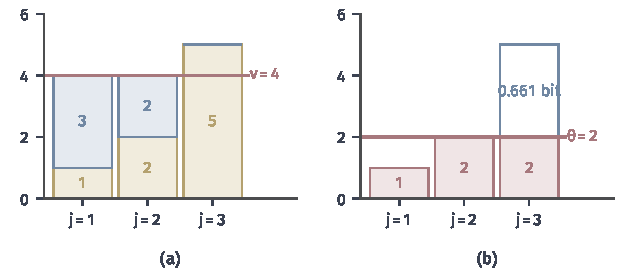
\includegraphics[width=106mm]{figures/07-probability/06-channel-coding/matplotlib/gcc-waterfilling/figure.pdf}
 \caption{两种“注水”的对照，三个分量的方差都是$(1,2,5)$。(a)平行高斯信道的功率分配，总功率$5$：黄色是噪声方差构成的底，蓝色是分到的功率，红线是水位$\nu=4$，功率为$(3,2,0)$。(b)第~\ref{chap:rate-distortion}章独立高斯分量的反注水，总失真$5$：红色是各分量的失真$\min\{\theta,\sigma_j^2\}$，红线是$\theta=2$，蓝框中高出$\theta$的部分需要描述，码率为$(0,0,0.661)$比特。}
 \label{fig:gcc-waterfilling}
\end{BookInlineFigure}

\paragraph{预算增加时}
水位随预算连续上升，分量按噪声从小到大依次加入。例中水位到达$2$时第二个分量开始分到功率，此时$P=\nu-1=1$；水位到达$5$时第三个分量加入，此时$P=(5-1)+(5-2)=7$。所以
\[
 P\leq1:\ \text{只用分量}1;\qquad 1<P\leq7:\ \text{用分量}1,2;\qquad P>7:\ \text{三个都用}.
\]
在每一段内，活跃分量的功率随$P$线性增长，斜率都是$1/a$，$a$是活跃分量数。图~\ref{fig:gcc-waterfill-path}(a)画出三条分配曲线，(b)比较三种分配方式的容量。

\begin{BookInlineFigure}
 \centering
 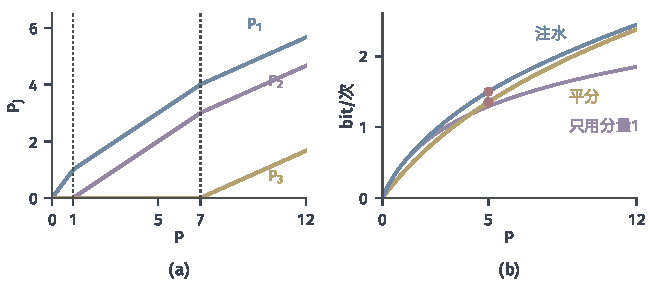
\includegraphics[width=110mm]{figures/07-probability/06-channel-coding/matplotlib/gcc-waterfill-path/figure.pdf}
 \caption{噪声方差为$(1,2,5)$时随总功率$P$的变化。(a)注水分配给三个分量的功率$P_1$（蓝）、$P_2$（紫）、$P_3$（黄），点线标出分量加入的位置$P=1$与$P=7$。(b)容量：注水分配（蓝）、平均分配（黄）、全部给分量$1$（紫）；红点是$P=5$时的$1.5$与$1.352$。}
 \label{fig:gcc-waterfill-path}
\end{BookInlineFigure}

乘子还有一层含义。由第~\ref{chap:discrete-channel-capacity}章成本约束下乘子的解释，$\mu$是预算的边际价值：总预算增加一个小量$\delta$，容量约增加$\mu\delta$。例中$\nu=4$，
\[
 \mu=\frac{1}{2\ln2\cdot4}=0.180\ \text{比特每单位功率}.
\]
直接验证：新增的功率平均分给两个活跃分量，每个水深增加$\delta/2$，每个分量的边际收益都是$1/(2\ln2\cdot4)$，容量增加约
\[
 2\cdot\frac{1}{2\ln2\cdot4}\cdot\frac{\delta}{2}=\mu\delta .
\]
第三个分量的起始边际收益是$1/(2\ln2\cdot5)=0.144$，低于$\mu=0.180$，这正是KKT条件中$\eta_3=\mu-0.144\geq0$的含义：把功率挪一点给它，只会得不偿失。

\paragraph{与反注水的对照}
第~\ref{chap:rate-distortion}章为独立高斯信源分配码率时也出现了一个“水位”，称为反注水：各分量的失真取$D_j=\min\{\theta,\sigma_j^2\}$，方差不超过$\theta$的分量不必描述。两种分配形式相似，分配的对象和方向却相反。图~\ref{fig:gcc-waterfilling}把它们并排画出，表~\ref{tab:gcc-water-vs-reverse}列出对应关系。

\begin{BookInlineTable}
 \centering
 \caption{注水与反注水的对照}
 \label{tab:gcc-water-vs-reverse}
 \begin{tabular}{lll}
  \toprule
   & 注水（信道） & 反注水（信源） \\
  \midrule
  分配的量 & 发送功率$P_j$ & 允许的失真$D_j$ \\
  分配规则 & $P_j=(\nu-\sigma_j^2)^{+}$ & $D_j=\min\{\theta,\sigma_j^2\}$ \\
  $\sigma_j^2$的含义 & 噪声方差 & 信源方差 \\
  被舍弃的分量 & 噪声高于水位 & 方差低于水位 \\
  目标 & 最大化容量 & 最小化码率 \\
  \bottomrule
 \end{tabular}
\end{BookInlineTable}

信道一侧，水倒在噪声上面，噪声越小的分量越先得到功率，因为同样的功率在那里换来更多的可区分性。信源一侧，水位以下是允许的失真，方差越大的分量越需要码率，方差小于水位的分量直接用均值重构即可。两种问题都把总资源按边际收益相等的原则分配，只是一个分配的是用来传送的资源，一个分配的是允许损失的量。

\subsection{并行传输的计量}
\label{sec:gcc-parallel-accounting}

式~\eqref{eq:gcc-parallel-capacity}是单次向量使用上的信息容量。它的单位、它与标量公式的关系，以及它是否也是块码的速率极限，需要分别说明。

\paragraph{一次向量使用}
一次使用同时占用$k$个实分量，容量计的是这$k$个分量合起来送出的比特数。例中$C=1.5$比特每次向量使用，折合每个实分量$0.5$比特；这两个数不能与单个实分量的公式~\eqref{eq:gcc-capacity}直接比较。比如把全部功率$5$放在一条噪声方差为$1$的标量信道上，得到$\frac12\log_2 6=1.292$比特每次使用，它比$1.5$小，比$0.5$大：前者比的是同一预算下“一条线路”与“三条线路”的总量，后者把三条线路的总量摊到了每条线路上。比较时要先说清楚：资源是什么（总功率还是每条线路的功率），计量单位是什么（每次向量使用还是每个实分量）。

复值信道就是$k=2$且两分量噪声相同的平行信道。两个噪声方差都是$\sigma^2/2$，注水的水位是$\nu=\sigma^2/2+P/2$，两分量平分功率，容量是
\[
 2\cdot\frac12\log_2\frac{\sigma^2/2+P/2}{\sigma^2/2}=\log_2\Bigl(1+\frac{P}{\sigma^2}\Bigr)\ \text{比特每次复值使用},
\]
这回答了第~\ref{sec:gcc-optimal-input}小节留下的问题：平分不是约定，而是最优分配。

\paragraph{可达性}
单次使用的容量能否被块码达到，回答与标量情形相同。

\begin{theorem}[平行信道的编码定理]
\label{thm:gcc-parallel-coding}
设分量数$k$固定，$P>0$，信道由式~\eqref{eq:gcc-parallel}给出，码满足约束~\eqref{eq:gcc-parallel-power}。低于式~\eqref{eq:gcc-parallel-capacity}中$C(P)$的速率都可达，且最大错误概率可以趋于零；平均错误概率趋于零的码列，其码率的上极限不超过$C(P)$。
\end{theorem}

可达性可以直接由标量结果拼出来。设$R<C(P)$，$(P_1,\dots,P_k)$是注水分配，活跃分量的集合记作$J$。因为$R<\sum_{j\in J}\frac12\log_2(1+P_j/\sigma_j^2)$，可以把$R$拆成$R=\sum_{j\in J}R_j$，使每个$R_j$严格小于第$j$个分量的标量容量。对每个$j\in J$，由定理~\ref{thm:gcc-coding}，存在第$j$个分量上满足功率约束$P_j$、码率至少$R_j$、最大错误概率$\lambda^{(j)}_{\max}\to0$的码；不活跃的分量始终发送零。

把各分量的消息组成向量$m=(m_j)_{j\in J}$，消息总数是各分量消息数之积，至少为$2^{nR}$。每条组合码字的总能量不超过$n\sum_jP_j=nP$。接收端在每个分量上独立解码，只要有一个分量判错，整条消息就判错；由并集界，最大错误概率不超过$\sum_{j\in J}\lambda^{(j)}_{\max}\to0$。

也可以不拆分，把第~\ref{sec:gcc-coding}小节的证明中的“字母”换成$k$维向量：码字在每个时刻独立地抽取$\mathcal{N}(0,P_j')$的各分量，信息密度是各分量信息密度之和，三类错误的估计逐字成立，只是能量和信息密度的平均对时刻和分量同时进行。这种做法说明向量信息密度的集中同样可以控制整组分量的联合判决。

\paragraph{逆定理}
逆向的论证与标量情形相同，只多一层对分量的求和。记$P_{i,j}=\frac1M\sum_mx_{i,j}(m)^2$为第$i$个时刻第$j$个分量在消息上的平均功率。Fano不等式和数据处理之后，与第~\ref{sec:gcc-coding}小节的第二步相同，得到
\[
 I(X^n;Y^n)\leq\sum_{i=1}^{n}F(P_{i,1},\dots,P_{i,k}),\qquad
 F(p_1,\dots,p_k)=\sum_{j=1}^{k}\frac12\log_2\Bigl(1+\frac{p_j}{\sigma_j^2}\Bigr) .
\]
$F$是凹函数，由Jensen不等式，$\sum_iF(\bm{p}_i)\leq nF(\bar{\bm{p}})$，其中$\bar{\bm{p}}$是各时刻分配向量的平均。约束~\eqref{eq:gcc-parallel-power}保证$\bar{\bm{p}}$的分量之和不超过$P$，所以$F(\bar{\bm{p}})\leq C(P)$。其余步骤与式~\eqref{eq:gcc-converse}相同。

论证依赖两个条件：分量数$k$固定，不随块长增长；噪声在时间上独立，且各分量的方差不随时刻改变。若$k$随$n$增长，或者噪声方差随时刻变化，就需要重新处理这里的大数律和单次上界。
